\documentclass[letterpaper,10pt]{article}

\usepackage{geometry}
\usepackage{hyperref}
\usepackage[nopostdot]{glossaries}
\usepackage[pdftex]{graphicx}
\usepackage{tikz}
\usepackage{wrapfig}
\geometry{textheight=8.5in, textwidth=6in}
\newenvironment{bottompar}{\par\vspace*{\fill}}{\clearpage}

\makeglossaries
\loadglsentries[main]{Glossary}

\title{Progress Report For RockSat-X Payload - Hephaestus}
\author{Helena~Bales, Amber~Horvath, and Michael~Humphrey\\ \\ CS461 - Fall 2016}

\parindent = 0.0 in
\parskip = 0.1 in

\begin{document}
\maketitle

\begin{abstract}
The \gls{osu} RockSat-X team shall be named Hephaestus.
The progress of our project shall be outlined in this document.
The mission requires that the \gls{payload}, an autonomous robotic arm, perform a series of motions to locate predetermined targets.
The hardware shall be capable of performing the motions to reach the targets.
The software shall determine the targets and send the commands to the hardware to execute the motion.
The combination of the hardware controlled by the software shall demonstrate Hephaestus's ability to construct small parts on orbit.
\end{abstract}

\begin{center}

\includegraphics[scale=.3]{logo}

Hephaestus Mission Logo
\end{center}

\begin{bottompar}
Approved By
\_\_\_\_\_\_\_\_\_\_\_\_\_\_\_\_\_\_\_\_\_\_\_\_\_\_\_\_\_\_\_\_\_\_\_\_\_\_\_\_\_\_\_\_\_\_\_\_\_\_\_\_\_\_\_\_\_\_\_\_\_\_\_
Date \_\_\_\_\_\_\_\_\_\_\_\_\_\_\_\_\_\_\_\_\_\_\_\_\_\_\_\_ \\


Approved By
\_\_\_\_\_\_\_\_\_\_\_\_\_\_\_\_\_\_\_\_\_\_\_\_\_\_\_\_\_\_\_\_\_\_\_\_\_\_\_\_\_\_\_\_\_\_\_\_\_\_\_\_\_\_\_\_\_\_\_\_\_\_\_
Date \_\_\_\_\_\_\_\_\_\_\_\_\_\_\_\_\_\_\_\_\_\_\_\_\_\_\_\_ \\


Approved By
\_\_\_\_\_\_\_\_\_\_\_\_\_\_\_\_\_\_\_\_\_\_\_\_\_\_\_\_\_\_\_\_\_\_\_\_\_\_\_\_\_\_\_\_\_\_\_\_\_\_\_\_\_\_\_\_\_\_\_\_\_\_\_
Date \_\_\_\_\_\_\_\_\_\_\_\_\_\_\_\_\_\_\_\_\_\_\_\_\_\_\_\_ \\


Approved By
\_\_\_\_\_\_\_\_\_\_\_\_\_\_\_\_\_\_\_\_\_\_\_\_\_\_\_\_\_\_\_\_\_\_\_\_\_\_\_\_\_\_\_\_\_\_\_\_\_\_\_\_\_\_\_\_\_\_\_\_\_\_\_
Date \_\_\_\_\_\_\_\_\_\_\_\_\_\_\_\_\_\_\_\_\_\_\_\_\_\_\_\_ \\
\end{bottompar}

\clearpage
\tableofcontents
\clearpage

\section{Introduction}
The Hephaestus Payload is a rocketry \gls{payload} that will fly onboard the 2016-2017 RockSat-X rocket. 
The rocket will be launched from Wallops Flight Facility filled with
student-made \glspl{payload}. 
The Hephaestus \gls{payload} will be made up of a \gls{deployable} arm and a video camera. The arm will perform 
a series of motions that will be recorded by the video camera and sensors. Following the experiment, the 
arm will retract back into the rocket. The Hephaestus mission will be Oregon State University's first 
space mission and will prove not only our ability to develop a space-ready
\gls{payload}, but also the 
viability of construction in space using a robotic arm.

\subsection{Document Overview}
This document will serve as a progress update following Fall term of 2016. At the time of writing, we 
have worked on the Hephaestus \gls{payload} for ten weeks. This document will include an overview of the 
project goals and purpose, our work so far, the problems we have encountered, and a retrospective.

\section{Project Overview}
\subsection{Project Purpose}
The Oregon State University RockSat-X team will demonstrate that an autonomous robotic arm can locate predetermined
 targets around the \gls{payload} under microgravity conditions by using precise movements. 
The technical actions performed by this demonstration will illustrate a proof of concept for creating assemblies, 
autonomous repairs, and performing experiments in space.
\subsection{Mission Success Criteria}
The Oregon State University RockSat-X team will demonstrate that an autonomous robotic arm can locate predetermined targets around the 
\gls{payload} under microgravity conditions by using precise movements. The technical actions performed by this demonstration will illustrate 
a proof of concept for creating assemblies, autonomous repairs, and performing experiments in space. 
The mission objectives are to deploy a robotic \gls{payload} capable of moving with four axes of freedom; deploy a Camera with a single axis 
of freedom;
enact a series of pre-scripted movements by the arm including contact with stationary sensors;
coordinate the Camera to track arm movements and record demonstration; and
store sensor data for when arm is at rest, and when it comes into contact with station sensors.
\section{Current Progress}
\subsection{Helena Balse}
\subsubsection{Week 3}
\begin{itemize}
\item{
\textbf{Progress}

This week I made significant strides in the design of our project. I wrote part of the Project Definition assignment. I started the Project Description with a description of the problem, broken down into the requirements of the RockSat-X program and the \gls{payload} that we decided on for the project. In order for our senior design project to be successful, we have to build the \gls{payload}, meet the RockSat-X project requirements (such as testing, documentation, and design reviews), and meet the capstone class requirements. Our \gls{payload} idea is a mechanical arm, and as a project it is capable of meeting all the requirements.

While the Project Definition document met our capstone class requirements for the week, there were also RockSat-X requirements to be met this week. The RockSat-X CoDR (Conceptual Design Review) was this week. As a large group (including two teams of ME's, one team of EE's, and the CS team) we developed the CoDR powerpoint that was presented yesterday to RockSat-X. This document included all of our conceptual \gls{payload} designs thus far, and was our first time presenting our designs to the RockSat-X group. Following that presentation, in order to meet the RockSat-X requirements, we took a group photo.

In addition to the RockSat-X requirements and the capstone class requirements,
we met the \gls{payload} requirements by meeting with Nancy Squires to discuss
the project, get approval of the Project Definition assignment, and discuss
starting an official Space Lab at \gls{osu}. The CoDR presentation is available here: 

https://github.com/balesh2/SeniorDesign/blob/master/presentations/CoDR-Hephaestus.pdf
}

\item{
\textbf{Plans}

The next week will be focusing on the development of documents for Senior Design class as well as for the RockSat-X project. Specifically, we will be revising the Project Description document and begin the Requirements Document. We will also be continuing the design process for the \gls{payload} with the other teams.
}

\item{
\textbf{Problems}

None.
}
\end{itemize}

\subsubsection{Week 4}
\begin{itemize}
\item{
\textbf{Progress}

This week I was at the Grace Hopper Celebration of Women in Computing. I did not do any work directly on the RockSat-X project, but I did talk to many people about Computer Science and space exploration.
}
\item{
\textbf{Plans}

Next week will be focusing on the development of the requirements document for Senior Design and PDR presentation. The PDR presentation is coming up and will require us to compile a powerpoint about our design, practice presenting it, and presenting it for the RockSat-X program.
}
\item{
\textbf{Problems}

I encountered a significant obstacle to completing work this week. I did not have internet access at Grace Hopper, so I was unable to work on the project or create an update.
}
\end{itemize}

\subsubsection{Week 5}
\begin{itemize}
\item{
\textbf{Progress}

This week was focused on developing the requirements document for Hephaestus and revising the Project Description document. The revision of the Project Description document was turned in on Wednesday after adding more of a focus on the software side of the project. The first draft of the requirements document will be turned in by the end of the day today. I focused on creating the outline of the document and writing the introduction. The introduction establishes a purpose and description of the document, an overview of the mission description, the mission success criteria, and the priorities for the requirements. The rest of the document describes the functional and non functional requirements that we have established for the software that controls the Hephaestus \gls{payload}.
}
\item{
\textbf{Plans}

The next week will focus on creating a solid final draft of the Requirements Document and presenting PDR. That will require meeting as a group to practice presenting PDR and meeting as a group to present PDR.
}
\item{
\textbf{Problems}

Availability has been a problem this week. It has been a challenge to fit all of the large group meetings into my schedule and still have time to catch up on homework after Grace Hopper and work.
}
\end{itemize}

\subsubsection{Week 6}
\begin{itemize}
\item{
\textbf{Progress}

This week, work focused on the development of the Requirements Document for Senior Design and finalizing the PDR presentation for RockSat-X. I mainly focused on the Requirements Document, and did significant work on the structure and content of that document. We turned in a draft first, then flushed it out to a final document that was turned in on Friday of Week 6. I focused on the functional requirements, introduction, and structure of the paper. For the PDR presentation, we had to develop requirements and a plan to meet the requirements. There was a lot of overlap in content between PDR and the Requirements Documents, which was ideal for finishing both of these big documents in the same week. In preparation for this presentation, we had one meeting where we all went over content and one where we practiced the presentation. The final presentation for PDR (Preliminary Design Review) was at 7am on Thursday of week 6. Finally, I revised the README for this repository, so that it was more informative regarding the structure, contents, and context of this repository.
}
\item{
\textbf{Plans}

Next week will focus on finalizing major design choices and developing the technical review. The design choices that need to be finalized include the method for assigning test points and the operational modes of the arm.
}
\item{
\textbf{Problems}

None.
}
\end{itemize}

\subsubsection{Week 7}
\begin{itemize}
\item{
\textbf{Progress}

This week we are developing the Technical Review Document for Senior Design. As such, we have divided the requirements up between the three of us as follows:

\textbf{Amber Horvath:}

    Emergency Expelling of Payload

    Program Modes of Operation

    Target Success Sensors

\textbf{Helena Bales:}

    Target Generation

    Movement of arm

    Arm position tracking

\textbf{Michael Humphrey:}

    Telemetry

    Video Camera

    Data visualization and processing

Each of us shall be responsible for insuring the completion of their assigned tasks. We will focus on our assigned tasks for the tech review. This week has focused on defining and assigning the requirements to each of us. We have also finalized some design choices, specifically in the modes of operations, emergency procedures, and arm target generation.
}
\item{
\textbf{Plans}

Next week we will complete and turn in the tech review on Monday of Week 8. Before that date we will be finishing that document. After the completion of the tech review we will be going back through past documents and including all suggestions we have received as feedback throughout the course. We will be doing this to prepare for the final document to be turned in on December 4th. We will also be preparing our designs and requirements for our big RockSat-X review during weeks 10 or 11.
}
\item{
\textbf{Problems}

We mainly are encountering the issue that we have too many assignments due on or before Monday of Week 8.
}
\end{itemize}

\subsubsection{Week 8}
\begin{itemize}
\item{
\textbf{Progress}

This week we finalized and turned in the technical review document. Preparing this document required meeting as a group to talk about potential solutions, then documenting the solutions that we came up with. This week we also talked to the Electrical Engineering group to make sure that our plans were consistent and that we would be able to work together on the software/hardware interface in the future.
}
\item{
\textbf{Plans}

Next week we plan on starting the Design Document and the presentation for the end of the term and our CDR presentation with RockSat-X.
}
\item{
\textbf{Problems}

I have been experiencing technical issues with my computers, so that is something that I will need to resolve before I can seriously start working on the Design Document.
}
\end{itemize}

\subsubsection{Week 9}
\begin{itemize}
\item{
\textbf{Progress}

This week we started the Design Document and slides for the presentation for this class and for our RockSat-X program CDR. We met in order to discuss the solutions that we wanted to choose for each of the requirements. During that meeting I updated our Design Document to reflect the choices that we made, and created issues to reflect the tasks that we have yet to complete.
}
\item{
\textbf{Plans}

In the next week we will be finishing the Design Document, finishing our slides for the class presentation, finishing our slides for the CDR presentation, practicing the CDR presentation, and starting to compile the progress update assignment.
}
\item{
\textbf{Problems}

I am still experiencing technical issues with my computer, but less seriously than before, so progress has been made there.
}
\end{itemize}

\subsubsection{Week 10}
\begin{itemize}
\item{
\textbf{Progress}

This week we finished up the Design Document and started the Progress Update write up and presentation. We also prepared for CDR by adding slides to the presentation. In order to finish the design document we talked about how to solve each of the issues from the Requirements document. Once we picked a solution to pursue, we each added detail to our solutions. The CDR presentation was adapted to form the start of our Progress Update presentation since it already describes the project and our work thus far.
}
\item{
\textbf{Plans}

Next week we will be finishing our progress update write up and presentation. We will do the write up first, then make sure that the presentation slides cover the content from the write up, and finally record the presentation.
}
\item{
\textbf{Problems}

None.
}
\end{itemize}

\subsection{Amber Horvath}
\documentclass[letterpaper,10pt]{article}
\title{Winter Progress Report for RockSat-X Payload - Hephaestus \\ Group 26}
\author{Amber~Horvath\\ \\ CS462 - Winter 2017}
\usepackage[pdftex]{graphicx}
\usepackage{tikz}
\usepackage{float}

\parindent = 0.0 in
\parskip = 0.1 in

\begin{document}
\maketitle

\section{Introduction}
The Hephaestus Payload is a rocketry payload that will fly onboard the 2016-2017 RockSat-X rocket. 
The rocket will be launched from the Wallops Flight Facility filled with student-made payloads from 
various institutions. The Hephaestus payload will consist of a deployable arm and a video camera.
The arm shall extend and move to a series of pre-placed sensors and make contact with the sensors. 
The arm will then contract and retract back into the rocket.
The video camera shall record the arm's movement. Data about the flight, such as error codes, shall be 
sent via a telemetry port and written onto a microSD card.
The Hephaestus mission will be Oregon State University's first space mission and will prove not only
our ability to develop a space-ready payload, but also the viability of construction in space using a robotic
arm.
\section{Individual Pieces}
The individual pieces of the project I am in charge of for the project include Emergency Retraction, 
Modes of Operation, and Touch Sensor Viability. I also took on the Data Storage task by the request
of the Electrical Engineering team.
\subsection{Emergency Retraction}
In the case of the arm getting caught in a bad state, we shall retract the arm back into a safe state
This will be accomplished by testing for a bad state.
We will retract the arm and test whether or not we?re in our calibrated normal position
If we are not, we are in a bad state and need to execute the emergency arm retraction.
We will then disable each motor except the one attached to the base of the payload.
Once each motor has been disabled, we will retract the base of the payload.
\subsection{Modes of Operation}

\begin{center}
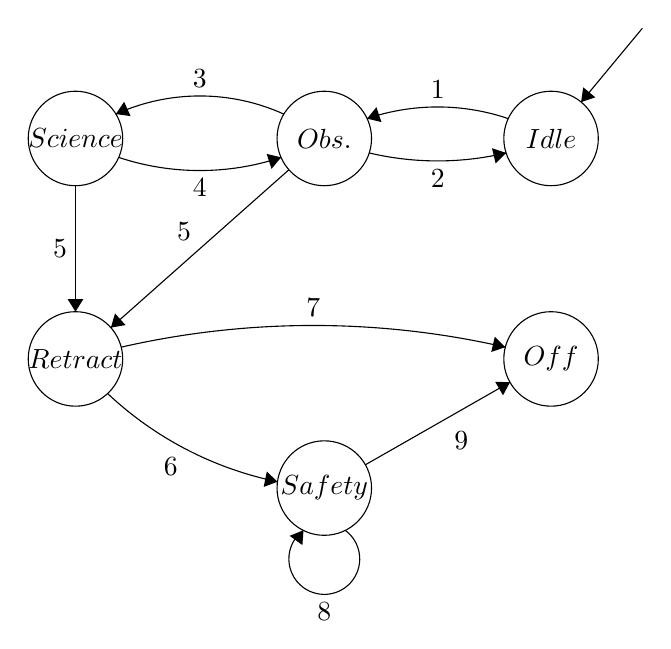
\begin{tikzpicture}[scale=0.2]
\tikzstyle{every node}+=[inner sep=0pt]
\draw [black] (46.2,-13.5) circle (3);
\draw (46.2,-13.5) node {$Idle$};
\draw [black] (31.8,-13.5) circle (3);
\draw (31.8,-13.5) node {$Obs.$};
\draw [black] (16,-13.5) circle (3);
\draw (16,-13.5) node {$Science$};
\draw [black] (16,-27.5) circle (3);
\draw (16,-27.5) node {$Retract$};
\draw [black] (46.2,-27.5) circle (3);
\draw (46.2,-27.5) node {$Off$};
\draw [black] (31.8,-35.7) circle (3);
\draw (31.8,-35.7) node {$Safety$};
\draw [black] (52,-6.5) -- (48.11,-11.19);
\fill [black] (48.11,-11.19) -- (49.01,-10.89) -- (48.24,-10.25);
\draw [black] (34.516,-12.239) arc (108.749:71.251:13.951);
\fill [black] (34.52,-12.24) -- (35.43,-12.46) -- (35.11,-11.51);
\draw (39,-11) node [above] {$1$};
\draw [black] (43.348,-14.419) arc (-76.68931:-103.31069:18.884);
\fill [black] (43.35,-14.42) -- (42.45,-14.12) -- (42.68,-15.09);
\draw (39,-15.43) node [below] {$2$};
\draw [black] (18.564,-11.955) arc (114.4174:65.5826:12.909);
\fill [black] (18.56,-11.95) -- (19.5,-12.08) -- (19.09,-11.17);
\draw (23.9,-10.3) node [above] {$3$};
\draw [black] (29.056,-14.702) arc (-71.60296:-108.39704:16.337);
\fill [black] (29.06,-14.7) -- (28.14,-14.48) -- (28.45,-15.43);
\draw (23.9,-16.04) node [below] {$4$};
\draw [black] (16,-16.5) -- (16,-24.5);
\fill [black] (16,-24.5) -- (16.5,-23.7) -- (15.5,-23.7);
\draw (15.5,-20.5) node [left] {$5$};
\draw [black] (29.55,-15.49) -- (18.25,-25.51);
\fill [black] (18.25,-25.51) -- (19.18,-25.35) -- (18.51,-24.61);
\draw (22.89,-20.01) node [above] {$5$};
\draw [black] (28.83,-35.296) arc (-101.59962:-133.25786:22.283);
\fill [black] (28.83,-35.3) -- (28.15,-34.65) -- (27.95,-35.63);
\draw (22.05,-33.75) node [below] {$6$};
\draw [black] (34.41,-34.22) -- (43.59,-28.98);
\fill [black] (43.59,-28.98) -- (42.65,-28.95) -- (43.15,-29.81);
\draw (40.5,-32.1) node [below] {$9$};
\draw [black] (33.123,-38.38) arc (54:-234:2.25);
\draw (31.8,-42.95) node [below] {$8$};
\fill [black] (30.48,-38.38) -- (29.6,-38.73) -- (30.41,-39.32);
\draw [black] (18.905,-26.751) arc (102.88102:77.11898:54.705);
\fill [black] (43.3,-26.75) -- (42.63,-26.09) -- (42.4,-27.06);
\draw (31.1,-24.87) node [above] {$7$};


\end{tikzpicture}
\end{center}



The Modes of Operation detail the states the program will be in during the course of the flight, as seen in the included state diagram. The transitions are as such:
\begin{enumerate}
\item{\textbf{Apogee is reached.} The experiment begins; the camera is powered on; and the on-board 
computer is on. A camera sweep is performed.}
\item{\textbf{Error: Return to Idle.} If an error occurs, we shall transition back to Idle mode.}
\item{\textbf{Payload Assembly and Camera have been deployed.} The software shall enter Science
mode once the payload assembly has been deployed and the camera sweep has completed.}
\item{\textbf{Error: Return to Observation.} If an error occurs, we transition back to Observation mode.}
\item{\textbf{Timer switch to end apogee period.} Experiment time has ended, proceed to Retract mode 
to prepare for descent.}
 \item{\textbf{Error: Proceed to Safety.} If the arm fails to retract, proceed to Safety mode.}
 \item{\textbf{Power off.} Arm is retracted, payload is retracted, computer is powered off, camera is 
 powered off. Payload is ready for descent.}
 \item{\textbf{Cycle in Safety.} Continually attempt to retract the arm and payload and power off the 
 computer and camera.}
 \item{\textbf{Power off.} Payload is now ready for descent.}
\end{enumerate}
\subsection{Touch Sensor Viability}
Within the body of the payload, two touch sensors will be placed at predetermined locations.
The arm shall make contact with the touch sensor and press it.
Upon being pressed, the touch sensor will go high and send a signal over telemetry and be written to
an SD card. The arm will then recalibrate before moving to the next sensor. If no sensors remain, 
the arm will retract and await shutdown.

\section{Progress and Problems}
\subsection{Emergency Retraction}
Due to the testing of emergency retraction being dependent upon the payload being assembled and the 
motors being attached to the payload, this has been a lower priority task. Pseudocode was written that 
details how this component of the project interacts with the other components of the program, but the 
code has not yet been completed. Code has been written for the interrupt subroutine that will notify the 
on-board computer to halt the current process and power off the specified motors.
\subsection{Modes of Operation}
The Modes of Operation requirement was technically completed last term, as it was essentially a state 
diagram that detailed how the program would operate throughout the flight. A state was added during the 
middle of the term to account for the time when the payload is being retracted from its extended state, 
but no other changes were made. As more code is being written, the modes of operation requirement will 
entail me ensuring that the design of the program upholds the design we originally developed last term.
\subsection{Touch Sensor Viability}
Similar to the Emergency Retraction requirement, due to dependencies of other components of the 
payload being assembled first, the Touch Sensor Viability requirement has been a lower-priority task. 
The dependences that must be resolved include determining the locations the arm will move to and 
implementing the code to move the arm to that location. Both those requirements are to be completed by 
Helena and her sub-team, "Pathing and Automation".
\subsection{Data Storage}
The Data Storage requirement has been the requirement that I have worked on the most the past term.
This is due to the other requirements having dependencies that must be resolved before progress
can be made, and the Electrical Engineers wanting this to be completed. The Data Storage component of the overall project has included numerous steps for completion including researching previous projects
similar to ours that required a micro controller and SD card, researching how SD cards work, requesting
assistance from experts around campus, and implementing the code and writing code specific to our ATMega128 and micoSD card. After researching solutions already in place for the larger question our team had ("How can you write data to an SD card from an ATMega128 micro controller?"), we chose to 
leverage the already-existing FatFS library, written by Elm-chan. The code is written in C and includes
a variety of files, some of which required ATMega128-specific code to be added in order to make it
compile and run. 

\begin{figure}[H]
\begin{center}
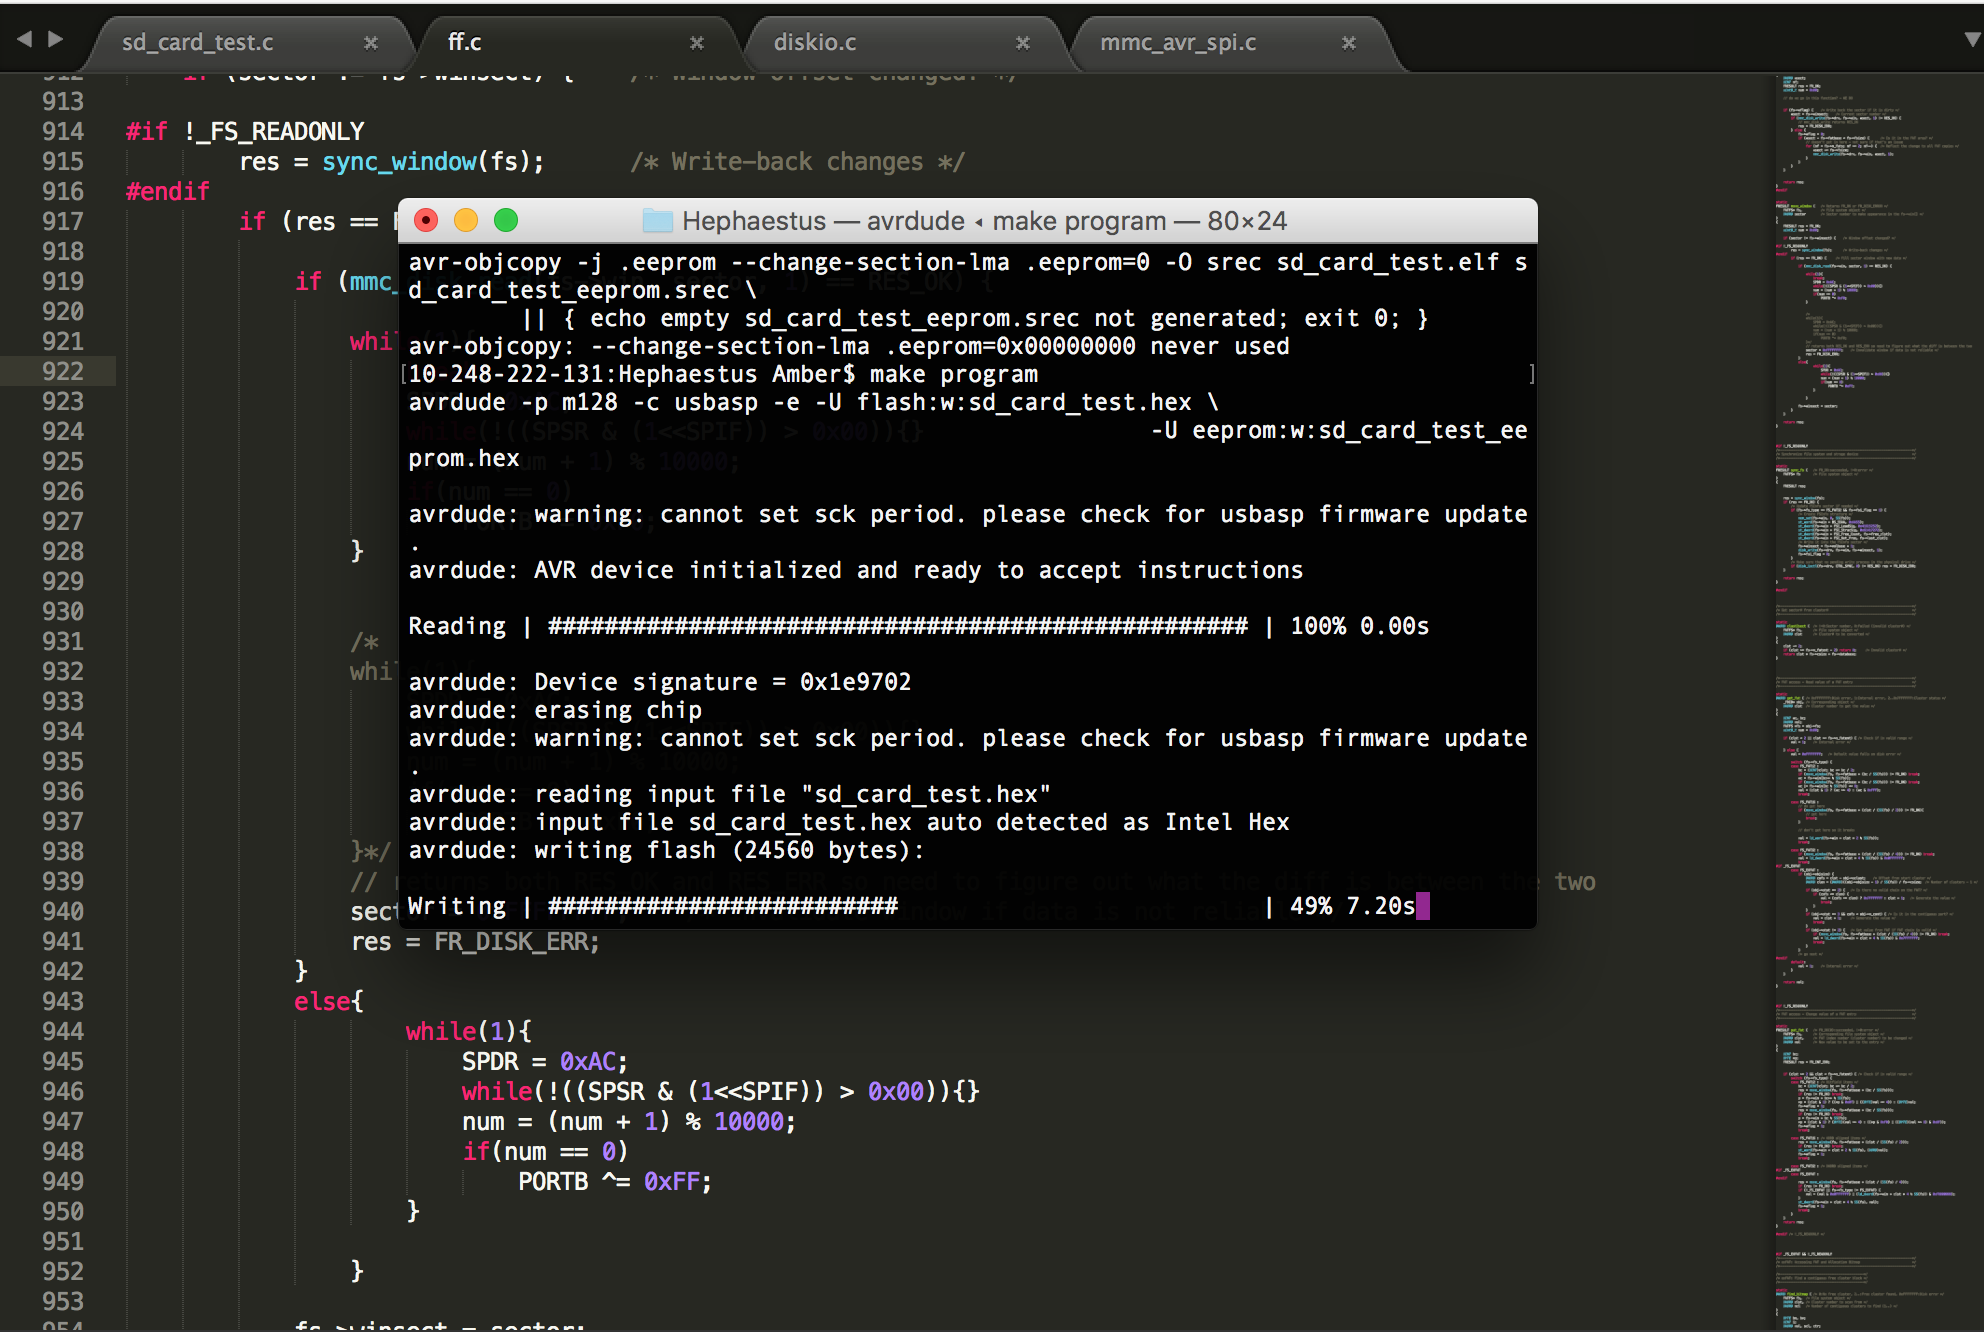
\includegraphics[height=5cm,width=\linewidth,keepaspectratio]{code.png}
\caption{An editor showing the files primarily used from the FatFS library and the code compiling with the avrdude compiler}
\label{fig:code}
\end{center}
\end{figure}
As shown in Figure \ref{fig:code}, there are 4 files currently open in the editor. One is "sdcardtest.c", 
which is the current file being used to test the core functionality our system requires. Our system must 
be able to open a file, write or append some data to the opened file, and close the file. 
These functionalities map to the API calls specified in "ff.c", the currently open file in Figure 
\ref{fig:code}. The main focus of my effort has been on getting these API calls to work as we intend
for them to. Currently, calls to the "fmount" function, which mounts the filesystem onto the micro
controller, and the "fopen" function, which creates a file pointer, work. However, we have not
been able to get writing to a file to work. This has been a large blocker for progress as the errors thrown
are difficult to follow and, as evident within Figure \ref{fig:code} there is a large amount of code that
must be sifted through, with many function calls leading to other parts of the library. Another layer
of complexity comes from the specificity of the problem, as there is documentation and forum
posts about using the FatFS library, but few that are as specific as using an ATMega128 with
a microSD card of our specific type.


\section{Evaluation}
Our team has had ups and downs this term. During the beginning of the term, we did not have a clearly
established workflow and felt minimal to no progress was being made, which caused a lot of stress
between all of us. Fortunately, we have put in systems such as mandatory group meetings and a scrum
update worksheet so we can ensure progress is being made. I believe our team will be a successful
development team as long as we continue adhering to these practices.
\subsection{Amber Horvath}
My main area of contribution has been on the Data Storage component as previously described.
I have put a lot of time and effort into this component and have collaborated with my peers,
namely Michael and our Electrical Engineer, Jonathan Hardman. I have also collaborated
with professors that are experts in this domain such as Roger Traylor. I am satisfied with the 
contribution to this team I've made over the course of the term. While I would've liked to
have the SD Card component fully completed by the end of this term, due to the nature of the
problem and the amount of work that is required to debug the program, I am trying to not be too hard on
 myself for not finishing this component. As for my role on the team, I feel I have fulfilled the duty of 
 keeping communication consistent and alive between team members. I have also tried to be a positive
 and empathetic member of the team so if spirits are getting low I try to get them back up. I feel
 the amount of work I have done is roughly equal to or above the other two members. This
 should be evident based on the blog post updates. However, it is hard to judge as a lot of our
 work has been collaborative and thus spread mainly evenly.
 \subsection{Helena Bales}
 Helena has filled the role of keeping the team focused and having the most expertise in the work
 we're doing. Due to her previous experience working with NASA and the UG Small Sat Lab, she
 is knowledgeable on more of the components of the project then myself. Overall, Helena's contribution
 to the team is probably lower or equal to myself and Michael's contribution. She was pivotal in the
 past couple weeks by mapping the Configuration Space and collaborating with the Pathing and
 Automation sub-team on that work, but it was harder to see progress being made prior to that point
 in the project. This is something our team could work on - having better communication between team
 members on progress or why progress is unable to occur.
 \subsection{Michael Humphrey}
 Michael has filled the role of keeping our information organized as he has been tasked with submitting
 group assignments. Michael has shown a commitment to staying on top of his workload and his
 level of organization has been an important asset to the team. I feel Michael's contribution to the
 project has been equivalent or less than mine. Michael worked on the Telemetry and Data Visualization
 component this term and showed progress, but not a largely significant amount. However, he did
 volunteer to help the Electrical Engineers and Mechanical Engineers on a testing component for their
 capstone classes which showed initiative that I appreciated. Overall, like Helena, I feel, due to the 
 nature of our project, towards the end of the term it was easier to see that he was making progress
 on his components of the project, but it would've been nice to know progress was being made
 all term.
 
\section{Retrospective}
\begin{center}
\begin{tabular}
%{ \textwidth }
{ | p{0.3\linewidth} | p{0.3\linewidth} | p{0.3\linewidth} | }
\hline
\textbf{Positives} & \textbf{Negatives} & \textbf{Changes} \\ \hline

We communicated with the larger team by holding weekly meetings. One person per team is required to represent the group at these meetings. & We did not take advantage of only one team member being required to attend the all-team meetings and usually had all three of our team members there. & We could change to usually only having two members attending, or not. \\ \hline

	We have established cross-functional team meetings. There are three cross functional teams, each with one member from the four main teams. The cross-functional teams meet once per week and report back to the rest of the groups. & The Electrical Integration team did not have much to talk about throughout this term due to delays in getting the motors. The Physical Integration team needed minimal software input so this time for the meeting could've been better utilized working on the project. & Motors have now been acquired, no further changes needed. \\ \hline

We asked for an extension on the progress update when we needed one. Asking for more time when we needed it was a goal that we set in last term's retrospective. & & We accomplished the change that we wanted to from last term, no further changes needed. \\ \hline

We learned about conflict resolution this term. & I (Helena) was not at my usual productivity and reliability levels, which put the rest of the team in an uncomfortable situation. I completed the work that I needed to, but did not communicate well enough with the rest of the team. & We talked as a group about how to resolve these issues and have improved our group dynamic and communication.\\ \hline

 & We were blocked from making progress on the technical side of the project for most of the term due to the delay in funding and receiving the motors. & In the future we should be more careful about parallelizing the technical tasks to decrease the affect of any blocks. \\ \hline

We a design review with the RockSat-X program office where we presented to a reviewer. This helped
us formally document the overall project. & Due to the time difference and the limitation of accomodating 16 schedules, we had to present at 6 AM
& We could stop whining about how early our design reviews always are. \\ \hline

We discussed the incorrect assumptions to get everyone on the same page 
& Occasional miscommunications between everyone regarding incorrect assumptions about the design
& Continue discussing misconceptions when they come up \\ \hline


\end{tabular}
\end{center}


\section{Conclusion}
In conclusion, I am greatly anticipating our next term and the continued success of our project. While 
this term was difficult and included some difficulties within our team, I believe in our ability to
 successfully carryout the remaining components of the project. I look forward to fully implementing
 the required programming components and seeing our fully assembled payload be able to move
 through space. I'm really excited about the work we're doing and to see our payload go into space!
 






\end{document}
\subsection{Michael Humphrey}
\subsubsection{Week 3}
This past week the Hephaestus project team accomplished several important milestones. We completed our first presentation to the RockSat-X organizers and took a group picture to start raising funding. We are also starting to narrow down our design for the final \gls{payload}.

Because the mechanical and electrical design of the project is not yet finalized, the software team has not yet had any important responsibilities. The electrical team is forbidden from using a device like a Raspberry Pi or an Arduino, so they have decided to use an AVR microcontroller. Amber and I have not used one of these devices, although Helena has. Amber and I will need to start doing research on programming for these devices. We will be using C to program the microcontroller. We won't be able to write any code until the electrical design (i.e. inputs and outputs) are finalized, but we can start creating a software design of how we want the software to work.

No problems have been encountered yet.

\subsubsection{Week 4}
Similar to week 3's blog post, this past week the Hephaestus Software Team did not have any major responsibilities. We attended the Hephaestus team meetings where the mechanical and electrical designs are still being worked out. We are going to have more communication with the Electrical Engineering team to determine the computing platform and computation restrictions. We also began working out budget numbers.

This next week we will be creating several presentations. I will be partly responsible for a 6 minute 40 second presentation to compete for a \$1,000 cash prize. Other fundraising efforts are also in progress. We will also be meeting with the Colorado Space Grant committee for our next presentation for them. We will also need to start working on revising our Problem Statement and start drafting our Requirements document and any other documentation we need.

Currently, the software team is blocked by the electrical team. Until they finalize a design, we cannot start coding. We will be in communication with them, however, to determine what considerations they need to take for the design.

\subsubsection{Week 5}
Since our mechanical and electrical design is still in progress, we have made no progress in the past week toward writing any software. Only work done was finishing the problem statement assignment and drafting our requirements document.

For the next week we will be getting datasheets and other information from the electrical team to aid in drafting our requirements documents. Any limitations of the hardware will be taken into consideration for the software requirements. Those materials should be made available by the electrical team by early next week.

Problems encountered this week were mostly personnel issues. Some of our team has been on vacation and one member is now sick and unable to make it on campus at all. I feel myself coming down with my second illness this term, which will make it even more difficult to get the required signatures we need.

\subsubsection{Week 6}
This week was spent finalizing our software requirements for the project. We did extensive research into the details of the mechanical and electrical design of our \gls{payload} and drew up documents with specifics such as coordinate systems and \gls{payload} layout. We now have a basis for creating our software.

For the next week, I believe we will be able to start writing the framework for the \gls{payload}. We probably won't be able to start programming the actual function of the \gls{payload} until it is built, but we can create the structure of how our software will be laid out.

Some problems were encountered this week with communication outside of our sub-team, but those have been resolved and shouldn't occur again in the future.

\subsubsection{Week 7}
Last week we developed the requirements of our system a lot. We explored technologies that we want to use and confirmed many details with the robotics and electronics team about the requirements of the \gls{payload}. For me, last week was spent primarily going to meetings, relaying information to teammates, and doing research into potential technologies we can use.

Next week, we will hopefully begin implementation of the software. I need to set up a meeting with the electrical team. I can't remember what they want to talk about but we definitely meet as a team with them. Most likely all of the CS team won't be able to make it, and this is a challenge we will need to overcome.

Problems I encountered included finding adequate solutions for the telemetry technology. I thought it would be easy to find several solutions we could use, but it turns out that most of the solutions I found were not compatible with our system for one reason or another. Mostly because none of them actually dealt with the transmission of the data itself, but what it did with the telemetry after it was collected. Other reasons were that they were implemented in the wrong language.

\subsubsection{Week 8}
Last week I helped start our Design Document. We've created the structure for the document and pasted the relevant sections from our previous documents. I set up meetings with the Electrical team and started communication with them to nail down specific software communication requirements. They're going to create a sort of "firmware" for the \gls{payload}, meaning they'll write the code that interacts directly with the hardware, and they'll expose an abstract interface for the Software team so we only need to call something like moveArm(x, y, z); to control the movement of the arm.

Next week we need to finalize the details of how we want to control the \gls{payload} arm. This will probably mean writing an API that we want the Electrical team to implement. We also need to prepare for the CDR coming up in a couple of weeks. This means we need to fill out the slides the Software team is responsible for. There will probably be other work for this presentation that we will tackle as it comes up.

No problems this week.

\subsubsection{Week 9}
This week I didn't do much. The Software team has created an outline for our design document but I haven't added my parts in. I don't foresee it being too much work, as it's mostly already written from the tech review. More details just need to be added. Due to it being Thanksgiving week, I have delayed working on classwork in favor of helping my family prepare for Thanksgiving.

Next week we need to finish our rough draft of the design document as well as write an outline for our presentation.

No problems were encountered this week.

\subsubsection{Week 10}
This week we made a lot of progress finalizing the design for the \gls{payload} software. This was mostly a result of writing the design document. There was much communication with the electrical team.

Next week is finals week. We will be writing our progress report and recording our presentation.

One problem we are encountered is the slow response to questions that arise about the RockSat-X program. I have several questions about the format and delivery of telemetry data that won't be answered until mid- to late-next week. That information was not able to be included in the design document.

\section{Retrospective}
\begin{center}
\begin{tabular}
%{ \textwidth }
{ | p{0.3\linewidth} | p{0.3\linewidth} | p{0.3\linewidth} | }
\hline
\textbf{Positives} & \textbf{Negatives} & \textbf{Changes} \\ \hline

We communicated with the larger team by holding weekly meetings. One person per team is required to represent the group at these meetings. & We did not take advantage of only one team member being required to attend the all-team meetings and usually had all three of our team members there. & We could change to usually only having two members attending, or not. \\ \hline

	We have established cross-functional team meetings. There are three cross functional teams, each with one member from the four main teams. The cross-functional teams meet once per week and report back to the rest of the groups. & The Electrical Integration team did not have much to talk about throughout this term due to delays in getting the motors. The Physical Integration team needed minimal software input so this time for the meeting could've been better utilized working on the project. & Motors have now been acquired, no further changes needed. \\ \hline

We asked for an extension on the progress update when we needed one. Asking for more time when we needed it was a goal that we set in last term's retrospective. & & We accomplished the change that we wanted to from last term, no further changes needed. \\ \hline

We learned about conflict resolution this term. & I (Helena) was not at my usual productivity and reliability levels, which put the rest of the team in an uncomfortable situation. I completed the work that I needed to, but did not communicate well enough with the rest of the team. & We talked as a group about how to resolve these issues and have improved our group dynamic and communication.\\ \hline

 & We were blocked from making progress on the technical side of the project for most of the term due to the delay in funding and receiving the motors. & In the future we should be more careful about parallelizing the technical tasks to decrease the affect of any blocks. \\ \hline

We a design review with the RockSat-X program office where we presented to a reviewer. This helped
us formally document the overall project. & Due to the time difference and the limitation of accomodating 16 schedules, we had to present at 6 AM
& We could stop whining about how early our design reviews always are. \\ \hline

We discussed the incorrect assumptions to get everyone on the same page 
& Occasional miscommunications between everyone regarding incorrect assumptions about the design
& Continue discussing misconceptions when they come up \\ \hline


\end{tabular}
\end{center}


\section{Conclusion}
The Hephaestus \gls{payload} will be Oregon State University's first space mission. 
It will prove the viability of construction in space using a mechanical arm 
capable of detailed maneuvers. The project is currently on schedule, with a 
launch in Summer of 2017. We have designed the software system to be applied to 
the hardware designed by the Mechanical Engineering teams and the Electrical 
Engineering team. During the course of this term, we encountered several 
problems, all of which we overcame through communication and time management. 
Following the completion of this term, the Hephaestus team will begin 
construction of the \gls{payload} and develoment of the software.


\clearpage
\printglossary[numberedsection]
\end{document}
